
\documentclass[13pt,compress]{beamer}
% deactivate beamer navigation
%\setbeamertemplate{navigation symbols}{}
%\usepackage{geometry}
%\geometry{papersize={180mm, 135mm}, top=-1.5mm} % 210mm, 297mm

\usepackage[nospeakermargin]{../../style/lmu-lecture}

\setbeamertemplate{frametitle}{\expandafter\uppercase\expandafter\insertframetitle}
%\useoutertheme{metropolis}
% remove section slides
\AtBeginSection[]
{
  \begin{frame}<beamer>
    \frametitle{Supervised Learning III}
    \tableofcontents[currentsection]
  \end{frame}
}
% includepdf slides, pagecommad will set counter for framenumber
\usepackage{pdfpages}
\includepdfset{trim=0mm 0mm 0mm 0mm, pagecommand={\global\setcounter{framenumber}{\value{page}}}}
% trim=0mm 6mm 0mm 0mm, offset=0 15,
% add footer:
\usepackage{framed, color}
\usepackage{xcolor}
%\iffalse
\usepackage{transparent}

\setbeamertemplate{footline}[text line]{%
    \noindent\hspace*{\dimexpr-\oddsidemargin-1in\relax}%
     \colorbox{white}{
     \makebox[\dimexpr\paperwidth-2\fboxsep\relax]{
     \color{black}
     \begin{minipage}[c][2.5ex][b]{0.5\linewidth}
       \secname
     \end{minipage}
     \hfill\begin{minipage}[c][2.5ex][b]{0.5\linewidth}
       \flushright
       \insertframenumber{}~/~\inserttotalframenumber~~
     \end{minipage}
     }}%
  \hspace*{-\paperwidth}
  }

%\fi

\title{Supervised Learning III}
\author{Essential Data Science Training}
%\institute{Essential Data Science Training}
\date{}



\begin{document}
\setbeamercolor{background canvas}{bg=}

% General remark: hyperlinks in included pdfs are not clickable anymore in the combined pdf

\frame{\titlepage}

\section{Gradient Boosting}
\includepdf[pages={2-4, 6-8}, trim=0mm 0mm 45mm 0mm]{../../material/lecture_sl/slides-pdf/slides-boosting-gradient-boosting-concept.pdf}
\includepdf[pages={2-8}, trim=0mm 0mm 45mm 0mm]{../../material/lecture_sl/slides-pdf/slides-boosting-gbm-with-trees-1.pdf}
\includepdf[pages={2-last}, trim=0mm 0mm 45mm 0mm]{../../material/lecture_sl/slides-pdf/slides-boosting-gbm-regularization.pdf}
\includepdf[pages={2, 5, 8-9}, trim=0mm 0mm 45mm 0mm]{../../material/lecture_sl/slides-pdf/slides-boosting-xgboost.pdf}
\section{Introduction to Feature Engineering}
\includepdf[pages={3-4}]{../../material/pdf_chapters/slides_intro_fe.pdf}
\includepdf[pages={1-last}]{../../material/pdf_chapters/slides_leakage.pdf}
\includepdf[pages={1-last}]{../../material/pdf_chapters/slides_ames_extended.pdf}
\section{Handling of Categorical Features}
\includepdf[pages={1-last}]{../../material/pdf_chapters/slides_categ_encode_dummy.pdf}
\includepdf[pages={1-last}]{../../material/pdf_chapters/slides_categ_encode_impact.pdf}
\section{Feature Transformation}
\includepdf[pages={1-last}]{../../material/pdf_chapters/slides_02_ftt_feature_trafos.pdf}
\section{Imputation}
\includepdf[pages={3-last}]{../../material/pdf_chapters/slides_01_imputation_intro.pdf}
\includepdf[pages={1-5}]{../../material/pdf_chapters/slides_02_imputation_simple.pdf}
\includepdf[pages={1-last}]{../../material/pdf_chapters/slides_03_imputation_models.pdf}
\section{Linear Pipelines with mlr3pipelines}
\includepdf[pages={4, 8, 10-13, 15-16, 18, 21, 25, 27-33, 36}]{../../material/mlr-doc/CURRENT_mlr3_course/03_mlr3pipelines/mlr3pipelines.pdf}
\section{Exercise: Simple Pipeline with mlr3pipelines}
\begin{frame}{Exercise: Simple Pipeline with mlr3pipelines}
\frametitle{Exercise: Simple Pipeline with mlr3pipelines} \footnotesize \begin{tabular}{|c|c|c|} \hline & \textbf{Topic} & \textbf{Filename} \\ \hline \textbf{Exercise / Demo} & Categorical Encoding & \textbf{day3\_encoding.html} \\ \hline \textbf{Homework (optional)} & Feature Transformation & \textbf{day3\_scaling.html} \\ \hline \end{tabular} 
\end{frame}

\section{Complex ML Pipelines with mlr3pipelines}
\includepdf[pages={59, 65-66, 49-51, 69-71, 73}]{../../material/mlr-doc/CURRENT_mlr3_course/03_mlr3pipelines/mlr3pipelines.pdf}
\section{Exercise: Complex Pipelines with mlr3pipelines}
\begin{frame}{Exercise: Complex Pipelines with mlr3pipelines}
\frametitle{Exercise (Homework): Complex Pipelines} \footnotesize \begin{tabular}{|c|c|c|} \hline & \textbf{Topic} & \textbf{Filename} \\ \hline \textbf{Homework (optional)} & Complex Pipeline & \textbf{day3\_impute\_filter\_tune.html} \\ \hline \end{tabular} 
\end{frame}




\end{document}
